\documentclass{scrartcl}

% Gráficos complejos
\usepackage{graphicx}
\usepackage{subfig}
\usepackage{placeins}

% Soporte para el lenguaje español
\usepackage{textcomp}
\usepackage[utf8]{inputenc}
\usepackage[T1]{fontenc}
\DeclareUnicodeCharacter{B0}{\textdegree}
\usepackage[spanish]{babel}

% Soporte para tablas avanzado
\usepackage{tabularx}
\usepackage[table]{xcolor}

% Formato de párrafo
\setlength{\parskip}{1ex plus 0.5ex minus 0.2ex}

% Formato de encabezados y pies de página
\usepackage{fancyhdr}
\fancyhead{}
\fancyfoot{}
\setlength\headheight{40pt}
\fancyhead[L]{
  Facultad de Ingeniería \\ 
  Universidad de Buenos Aires
}
\fancyhead[R]{
  75.09 - Análisis de la Información \\
  Trabajo Práctico - ShoppyCard \\
  Grupo 4
}
\fancyfoot[C]{
  \thepage
}
\pagestyle{fancy}

% Título
\title{75.09 - Análisis de la Información}
\subtitle{Trabajo Práctico - ShoppyCard - Grupo 4}
\date{}
\author{}

% Documento
\begin{document}

% Titulo e indice
\maketitle
\tableofcontents
\clearpage

% Secciones del documento
\part{Modelo de negocio}
\section{Objetivo}

 Administrar la operación de la tarjeta de crédito Shoppycard y emitir resúmenes.


\section{Alcance}

En las siguientes secciones se detallan los procesos de negocio alcanzados por
el proyecto, así como una pequeña descripción de cada uno de ellos.

\subsection{Emisión de nuevas tarjetas}

Registración de la solicitud de una nueva tarjeta, la validación de la misma y
la registración de la nueva tarjeta emitida, cuando correspondiese.

\subsection{Reemisión de tarjetas}

Modificación de las cuentas de los clientes registrados para asociarlas a una
tarjeta diferente de la entregada al procesar la solicitud de nueva tarjeta.

\subsection{Autorización de compras}

Autorización de una compra utilizando la tarjeta en un comercio, determinando si
dicha compra puede realizarse o no de acuerdo al saldo adeudado por el cliente y
otras reglas de negocio.

\subsection{Registración de compras}

Registración de los saldos diarios informados por los comercios para los pagos
realizados durante el día utilizando la tarjeta.

\subsection{Generación de resúmenes de cuenta de clientes}

Generación de reportes y resúmenes del saldo adeudado y movimientos mensuales
por cliente registrado, incluyendo reglas de cálculo de intereses por pagos
atrasados.

\subsection{Generación de resúmenes de cuenta de comercios}

Generación de reportes y resúmenes del saldo adeudado y movimientos mensuales de
los consumos para todos los clientes por comercio, incluyendo reglas de cálculo
de comisiones.

\subsection{Registración de pagos de clientes}

Registración de pagos individuales realizados por los clientes en concepto de
los resúmenes de cuenta por los movimientos realizados.

\subsection{Renovaciones de tarjetas}

Renovación automática de las tarjetas de crédito, anualmente, así como la
administración de la solicitud de cancelación de renovación.


\section{Hipótesis y supuestos}

En lo próximo se enumeran las hipótesis y otros supuestos tomados como
verdaderos para realizar el análisis subsiguiente detallado en lo que resta del
presente documento.

\subsection{Cancelación de tarjetas}

No se puede dar de baja una tarjeta una vez adquirida. Sólo se puede cancelar la
renovación de la misma, de modo que una vez pasado el periodo de expiración
determinado para cada tarjeta el proceso de renovación automática no se llevará
a cabo en dicha tarjeta.

La cancelación de la renovación invalida la tarjeta para efectuar consumos una
vez la tarjeta expira. De ninguna manera dicha cancelación es aplicable a los
saldos adeudados al día de la expiración, así como tampoco a los intereses
devenidos en las deudas acumuladas y no saldadas subsiguientemente.

Se continuarán emitiendo resúmenes de cuenta de clientes mensuales para aquellas
tarjetas canceladas que adeuden saldo. Sólo cuando la tarjeta no registre saldo
se dejarán de emitir resúmenes mensuales.

\subsection{Límite de consumo}

Las cuentas de los clientes tienen un límite de saldo fijo, determinado al momento de su creación. No se autorizarán movimientos cuando estos hagan superar dicho límite.

\subsection{Cálculo de intereses}

Se aplicará un interés fijo del 5 \% mensual si el monto adeudado por cada
cliente no es abonado antes del día 10 de cada mes. Dicho interés pasa a ser
entonces parte de la deuda, y es elegible al mes siguiente para generar
intereses del mismo modo que los montos correspondientes a los consumos.

\subsection{Envío de resúmenes}

No se contemplará ningún tipo de mecanismo para entregar el resumen mensual de
consumos a los comercios ni el resumen mensual de cuenta a los clientes.

\subsection{Pagos a comercios}

El primer día de cada mes se emitirá un reporte de saldos adeudados por
comercio, indicando el monto que se le debe pagar a cada uno de ellos por los
consumos realizados por los distintos clientes durante el mes anterior. Sobre
este monto se descontará un 5\% de comisión sobre el monto bruto total.

No se contemplará ningún medio para registrar los pagos realizados a los
comercios por estos conceptos en este proyecto. Se recomienda considerar
implementar un sistema de facturación más completo para controlar estos pagos.

\subsection{Registración de ventas}

No se contemplará ningún tipo de control en la interacción de los procesos de
autorización de compras e información de ventas por parte de los comercios
adheridos. Se supone que no se realizará una venta sin autorizarla primero. Por
consiguiente, dichos procesos son independientes.

\section{Diagramas de actividades}

A continuación se presenta una serie de diagramas de actividades que sumarizan
los diversos procesos alcanzados por el proyecto. Primeramente se presenta un
diagrama de actividades unificado que describe todos los procesos alcanzados.
Seguidamente, se exponen varios diagramas adicionales con los detalles de cada
uno de ellos.

\begin{figure}[htb]
\begin{center}
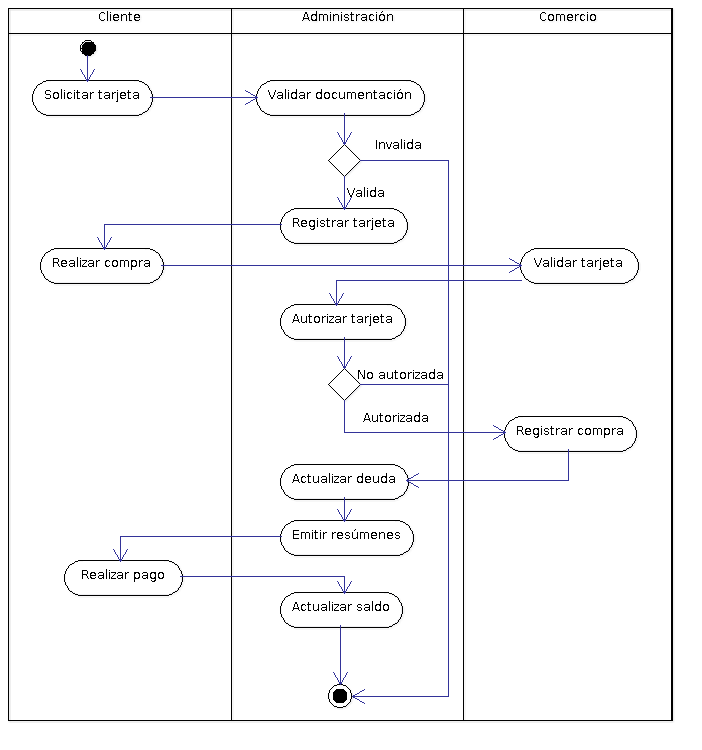
\includegraphics[width=\textwidth]{images/mod_negocio_act_global.png}
\end{center}
\caption{Diagrama de actividades general de los procesos alcanzados por el
proyecto.}
\end{figure}

\begin{figure}[htb]
\begin{center}
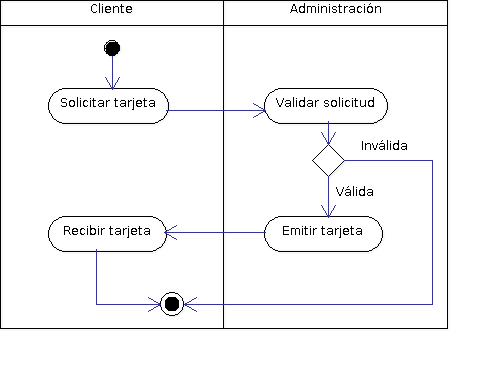
\includegraphics[width=0.7\textwidth]{images/mod_negocio_act_solicitudtarjeta.png}
\end{center}
\caption{Diagrama de actividades para el proceso de solicitud de una nueva
tarjeta.}
\end{figure}

\begin{figure}[htb]
\begin{center}
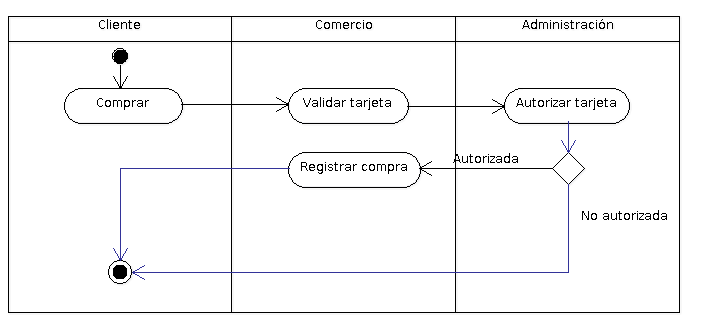
\includegraphics[width=0.9\textwidth]{images/mod_negocio_act_compra.png}
\end{center}
\caption{Diagrama de actividades para el proceso realización de una compra. El
comercio vende un producto y/o servicio a un cliente, quien opta por pagar por
este utilizando la tarjeta ShoppyCard.}
\end{figure}

\begin{figure}[htb]
\begin{center}
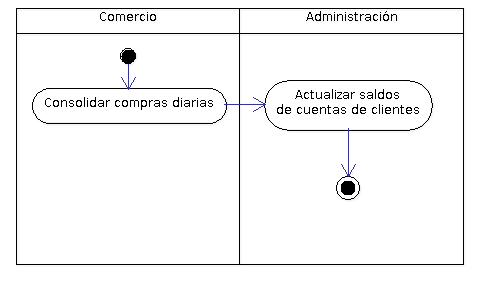
\includegraphics[width=0.7\textwidth]{images/mod_negocio_act_regcompras.png}
\end{center}
\caption{Diagrama de actividades para el proceso de actualización de saldos de
clientes. Diariamente, el comercio consolida la información de las compras
realizadas durante ese día y la envía a la administración.}
\end{figure}

\begin{figure}[htb]
\begin{center}
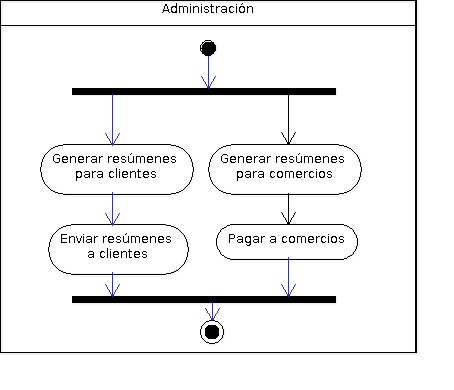
\includegraphics[width=0.7\textwidth]{images/mod_negocio_act_resumenes.png}
\end{center}
\caption{Diagrama de actividades para el proceso de emisión de resúmenes.
Mensualmente se generan los resúmenes de cuenta para los clientes, que son
enviados a cada cliente, y los resúmenes de saldo de cada comercio, utilizados
para realizar los pagos correspondientes.}
\end{figure}

\begin{figure}[htb]
\begin{center}
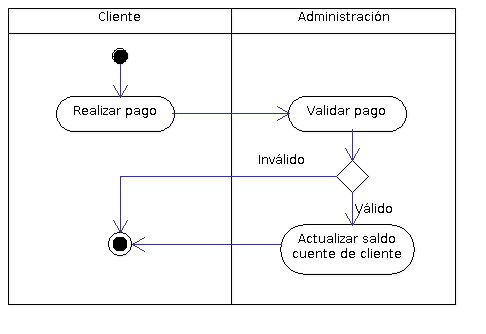
\includegraphics[width=0.7\textwidth]{images/mod_negocio_act_pago.png}
\end{center}
\caption{Diagrama de actividades para el proceso de pago. Del 1 al 10 de cada
mes, el cliente realiza el pago del importe detallado en el resumen que
recibió.}
\end{figure}

\FloatBarrier


\part{Modelo de casos de uso}
\section{Actores}

A continuación se describen los actores que se involucran, de una manera u otra,
con el sistema.

\begin{description}

\item[Cliente] \hfill \\
Solicita una tarjeta y realiza compras con ella.

\item[Comercio] \hfill \\
Realiza ventas de bienes y/o servicios al cliente, quien paga por ellos
utilizando la tarjeta.

\item[Administrador] \hfill \\
Configura y adminstra el sistema informático desarrollado manteniendo datos de
referencia como ser los comercios y clientes registrados.

\item[Mensualmente] \hfill \\
Actor temporal mensual involucrado en los procesos de generación de resúmenes de
cuenta por clientes y resúmenes de saldo por comercio.

\item[Diariamente] \hfill \\
Actor termporal diario involucrado en los procesos de verificación y renovación
de tarjetas vencidas.

\end{description}

\section{Diagrama de casos de uso} \label{sec:diagrama_casos_uso}

En la figura~\ref{fig:modcasosuso:diagramacasos} se exponen los actores
involucrados en la operación del sistema y su interacción con el mismo a través
de los casos de uso identificados. En secciones subsiguientes se detallará cada
uno de estos últimos.

\begin{figure}[htb]
\begin{center}
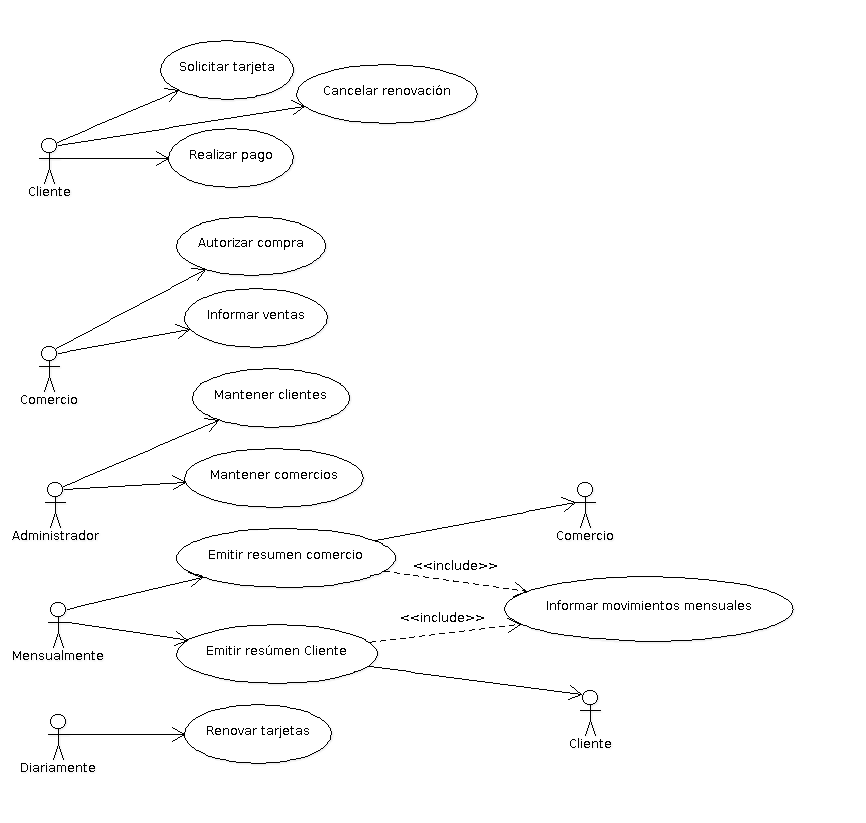
\includegraphics[width=0.9\textwidth]{images/mod_casosuso_diagrama.png}
\end{center}
\caption{Diagrama de casos de uso}
\label{fig:modcasosuso:diagramacasos}
\end{figure}

\FloatBarrier

\section{Detalle de casos de uso}

En esta sección se detallan cada uno de los casos de uso presentados en el
diagrama de casos de uso de la sección~\ref{sec:diagrama_casos_uso}.

\subsection{Solicitar tarjeta}
\begin{tabularx}{\textwidth}{| r | X |}
\hline
\multicolumn{2}{|X|}{
\textbf{Use Case}: Solicitar tarjeta} \\

\hline
\multicolumn{2}{|c|}{\cellcolor[gray]{0.6}} \\

\hline
\multicolumn{2}{|X|}{
\textbf{Descripción}: Registración de los datos de un cliente y emisión de una
tarjeta a su nombre.} \\

\hline
\multicolumn{2}{|X|}{
\textbf{Actores participantes}: Cliente} \\

\hline
\multicolumn{2}{|c|}{\cellcolor[gray]{0.6} } \\

\hline
\multicolumn{2}{|X|}{
\textbf{Flujos}} \\

\hline
\multicolumn{2}{|X|}{
\textbf{Flujo principal}} \\

\hline
1 & El cliente solicita una nueva tarjeta. \\
\hline
2 & El sistema solicita los datos del cliente. \\
\hline
3 & Se ingresan los datos del cliente (nombre, apellido, dni, límite de compra,
domicilio, teléfono). \\
\hline
4 & El sistema valida que el dni del cliente no haya sido registrado aún (E1.1
si ya ha sido registrado). \\
\hline
5 & El sistema pide confirmación de que el cliente ha presentado una fotocopia
de su dni (E2.1 si no se da confirmación). \\
\hline
6 & El sistema pide confirmación de que el cliente ha presentado la
documentación asociada a la garantía, y que esta es satisfactoria (E2.1 si no se
da confirmación). \\
\hline
7 & El sistema almacena los datos del cliente y genera un número de tarjeta. \\
\hline
8 & Fin del caso de uso. \\

\hline
\multicolumn{2}{|X|}{
\textbf{Flujos de excepción}} \\

\hline
E1.1 & El sistema emite un mensaje de error informando que el cliente ya posee
una tarjeta. \\
\hline
E1.2 & El caso de uso continua en 8 \\

\hline
E2.1 & El sistema emite un mensaje de error informando que el cliente no
presentó documentación obligatoria para continuar con la solicitud. \\
\hline
E1.2 & El caso de uso continua en 8 \\

\hline
\end{tabularx}



\subsection{Cancelar renovación}
\begin{tabularx}{\textwidth}{| r | X |}
\hline
\multicolumn{2}{|X|}{
\textbf{Use Case}: Cancelar renovación} \\

\hline
\multicolumn{2}{|c|}{\cellcolor[gray]{0.6}} \\

\hline
\multicolumn{2}{|X|}{
\textbf{Descripción}: Cancela el proceso de renovación automática de la tarjeta,
de manera que la tarjeta sigue vigente hasta que expire. A partir de su
expiración, la tarjeta se mantiene como inactiva y no puede ser utilizada.} \\

\hline
\multicolumn{2}{|X|}{
\textbf{Actores participantes}: Cliente} \\

\hline
\multicolumn{2}{|c|}{\cellcolor[gray]{0.6} } \\

\hline
\multicolumn{2}{|X|}{
\textbf{Flujos}} \\

\hline
\multicolumn{2}{|X|}{
\textbf{Flujo principal}} \\

\hline
1 & El cliente solicita la cancelación de la renovación automática de su
tarjeta. \\
\hline
2 & El sistema solicita el número de tarjeta del cliente. \\
\hline
3 & El sistema valida que el número de tarjeta del cliente exista (E1.1 si no
existe). \\
\hline
4 & El sistema valida que la tarjeta del cliente esté activa y su renovación no
haya sido cancelada (E2.1 si está inactiva o su renovación ya ha sido
cancelada). \\
\hline
5 & El sistema marca la tarjeta como "no renovar". Se mantiene activa, pero en
su fecha de expiración la tarjeta no se renovará automáticamente. \\
\hline
6 & Fin del caso de uso. \\

\hline
\multicolumn{2}{|X|}{
\textbf{Flujos de excepción}} \\

\hline
E1.1 & El sistema emite un mensaje de error informando que no existe una tarjeta
con el número de tarjeta ingresado \\
\hline
E1.2 & El caso de uso continua en 6 \\

\hline
E2.1 & El sistema emite un mensaje de error informando que la tarjeta está
inactiva o que su renovación ya ha sido cancelada. \\
\hline
E2.2 & El caso de uso continua en 6 \\

\hline
\end{tabularx}



\subsection{Realizar pago}
\begin{tabularx}{\textwidth}{| r | X |}
\hline
\multicolumn{2}{|X|}{
\textbf{Use Case}: Realizar pago} \\

\hline
\multicolumn{2}{|c|}{\cellcolor[gray]{0.6}} \\

\hline
\multicolumn{2}{|X|}{
\textbf{Descripción}: Registración de un pago a nombre de un cliente en
concepto de los consumos realizados durante el mes anterior.} \\

\hline
\multicolumn{2}{|X|}{
\textbf{Actores participantes}: Cliente} \\

\hline
\multicolumn{2}{|c|}{\cellcolor[gray]{0.6} } \\

\hline
\multicolumn{2}{|X|}{
\textbf{Flujos}} \\

\hline
\multicolumn{2}{|X|}{
\textbf{Flujo principal}} \\

\hline
1 & El cliente se presenta en las oficinas de pagos para pagar el monto
adeudado. \\
\hline
2 & El sistema solicita el DNI del cliente. (E1 si el cliente no existe). \\
\hline
3 & El sistema informa los datos del cliente para su validación, y solicita
confirmación de que estos son correctos (E2 si los datos no son correctos). \\
\hline
4 & El sistema informa el monto adeudado por el cliente. (S1 si el monto
adeudado es cero, S2 si la fecha del día no es del uno al diez de cada mes). \\
\hline
5 & El sistema solicita el importe abonado por el cliente y actualiza el saldo
de su cuenta corriente.\\
\hline
6 & Fin del caso de uso. \\

\hline
\multicolumn{2}{|X|}{
\textbf{Flujos alternativos}} \\

\hline
S1.1 & El sistema emite un mensaje informando que el cliente no posee saldo
adeudado. \\
\hline
S1.2 & El caso de uso continua en 6. \\

\hline
S2.1 & El sistema emite un mensaje informando que no se pueden registrar pagos
fuera de término, e indicando el próximo periodo en el que se podrán registrar
pagos (en las fechas uno al diez de cada mes). \\
\hline
S2.2 & El caso de uso continua en 6. \\


\hline
\multicolumn{2}{|X|}{
\textbf{Flujos de excepción}} \\

\hline
E1.1 & El sistema emite un mensaje de error informando que el cliente no
existe. \\
\hline
E1.2 & El caso de uso continua en 6. \\

\hline
E2.1 & El sistema emite un mensaje de error informando que no se registrará
ningún pago. \\
\hline
E2.2 & El caso de uso continua en 2. \\

\hline
\end{tabularx}



\subsection{Autorizar compra}
\begin{tabularx}{\textwidth}{| r | X |}
\hline
\multicolumn{2}{|X|}{
\textbf{Use Case}: Autorizar compra} \\

\hline
\multicolumn{2}{|c|}{\cellcolor[gray]{0.6}} \\

\hline
\multicolumn{2}{|X|}{
\textbf{Descripción}: Validación de las condiciones de uso de una tarjeta para
realizar un pago en un comercio adherido.} \\

\hline
\multicolumn{2}{|X|}{
\textbf{Actores participantes}: Comercio} \\

\hline
\multicolumn{2}{|c|}{\cellcolor[gray]{0.6} } \\

\hline
\multicolumn{2}{|X|}{
\textbf{Flujos}} \\

\hline
\multicolumn{2}{|X|}{
\textbf{Flujo principal}} \\

\hline
1 & El comercio requiere al sistema que este valide una tarjeta informando el
número de esta, el DNI del cliente y el importe de la venta que el cliente
quiere abonar utilizando la misma. \\
\hline
2 & El sistema realiza las siguientes validaciones (S1 si alguna de las
validaciones fallase). 
\begin{enumerate}
\item El número de tarjeta debe estar asociado a una tarjeta.
\item La tarjeta debe estar activa.
\item El DNI del cliente asociado a la tarjeta debe coincidir con el DNI
informado.
\item El saldo de la cuenta asociada a la tarjeta más el importe informado de
la venta no debe superar el límite de saldo asociado a la cuenta.
\end{enumerate} \\
\hline
3 & El sistema informa al comercio que la compra está autorizada. \\
\hline
4 & Fin del caso de uso. \\

\hline
\multicolumn{2}{|X|}{
\textbf{Flujos alternativos}} \\

\hline
S1.1 & El sistema informa al comercio que la compra no está autorizada,
adjuntando en el mensaje el motivo por el cual no se autoriza la misma. \\
\hline
S1.2 & El caso de uso continua en 4. \\

\hline
\end{tabularx}



\subsection{Informar ventas}
\begin{tabularx}{\textwidth}{| r | X |}
\hline
\multicolumn{2}{|X|}{
\textbf{Use Case}: Informar ventas} \\

\hline
\multicolumn{2}{|c|}{\cellcolor[gray]{0.6}} \\

\hline
\multicolumn{2}{|X|}{
\textbf{Descripción}: Registración de las ventas sumarizadas por día en un
comercio particular.} \\

\hline
\multicolumn{2}{|X|}{
\textbf{Actores participantes}: Comercio} \\

\hline
\multicolumn{2}{|c|}{\cellcolor[gray]{0.6} } \\

\hline
\multicolumn{2}{|X|}{
\textbf{Flujos}} \\

\hline
\multicolumn{2}{|X|}{
\textbf{Flujo principal}} \\

\hline
1 & El comercio informa las ventas realizadas a los distintos clientes en un
día particular, proporcionando la fecha para la cual se están informando las
ventas, el código del comercio que las está informando y un listado que indica
el número de tarjeta y el importe sumarizado de todas las ventas en la fecha
informada para dicha tarjeta.\\
\hline
2 & El realiza las siguientes validaciones (E1 si alguna de ellas fallase). 
\begin{enumerate}
\item Debe existir un comercio con el código de comercio informado.
\item La fecha proporcionada debe corresponder al mes actual.
\item Los números de tarjeta proporcionados deben estar todos asociados cada
uno a una tarjeta activa.
\end{enumerate}
\\
\hline
3 & El sistema registra las transacciones informadas. \\
\hline
4 & Fin del caso de uso. \\

\hline
\multicolumn{2}{|X|}{
\textbf{Flujos de excepción}} \\

\hline
E1.1 & El sistema emite un mensaje de error informando que los datos informados
son incorrectos, adjuntando un mensaje que indica la validación que falló. \\
\hline
E1.2 & El caso de uso continua en 4. \\

\hline
\end{tabularx}



\subsection{Mantener clientes}
\begin{tabularx}{\textwidth}{| r | X |}
\hline
\multicolumn{2}{|X|}{
\textbf{Use Case}: Mantener clientes} \\

\hline
\multicolumn{2}{|c|}{\cellcolor[gray]{0.6}} \\

\hline
\multicolumn{2}{|X|}{
\textbf{Descripción}: Mantenimiento de la información relacionada a los
clientes.} \\

\hline
\multicolumn{2}{|X|}{
\textbf{Actores participantes}: Administrador} \\

\hline
\multicolumn{2}{|c|}{\cellcolor[gray]{0.6} } \\

\hline
\multicolumn{2}{|X|}{
\textbf{Flujos}} \\

\hline
\multicolumn{2}{|X|}{
\textbf{Flujo principal}} \\

\hline
1 & El sistema solicita el DNI, nombre, apellido o teléfono del cliente. \\
\hline
2 & El administrador proporciona cualquier combinación de los campos
solicitados (por ejemplo, proporcionando nombre y apellido, o sólo nombre, o
teléfono y DNI, etc.). \\
\hline
3 & El sistema valida que se haya proporcionado información en al menos uno de
los campos (E1 si no se proporcionó ninguna información). \\
\hline
4 & El sistema realiza una búsqueda de todos los clientes registrados cuya
información coincida, aunque sea parcialmente, con los datos proporcionados. \\
\hline
5 & El sistema muestra un listado con todos los clientes cuya información
coincide, al menos parcialmente, con la información proporcionada. Dicho
listado debe incluir DNI, nombre, apellido y teléfono del cliente. Por cada
cliente, el sistema proporciona la opción de modificar dicha información. (S1
si el administrador elige la opción de modificar el cliente). \\
\hline
6 & Fin del caso de uso. \\

\hline
\multicolumn{2}{|X|}{
\textbf{Flujos alternativos}} \\

\hline
S1.1 & El sistema solicita el nombre, apellido, DNI, límite de compra,
domicilio, teléfono y número de tarjeta, completando por defecto cada campo con
el valor almacenado actualmente en el sistema para el cliente. \\
\hline
S2.1 & El sistema almacena los nuevos valores de cada campo para el cliente. \\
\hline
S1.2 & El caso de uso continua en 6. \\

\hline
\end{tabularx}




\part{Glosario}
\begin{description}

\item[Administración] \hfill \\
Grupo de trabajo encargado de la administración de todo lo relacionado a la
operación de la tarjeta ShoppyCard, incluyendo el personal de atención al
cliente, administradores del sistema informático ShoppyCard, encargados de pagos
y cualquier otro personal pertinente.

\item[Cliente] \hfill \\
Persona que adquiere productos y/o servicios en los comercios del centro
comercial.

\item[Comercio] \hfill \\
Entidad ubicada dentro del centro comercial que vende productos y/o servicios y
permite a aquellos que los adquieren utilizar la tarjeta ShoppyCard como forma
de pago por la adquisición de los mismos.

\end{description}


\end{document}

